\documentclass[10pt,twocolumn]{article}

\usepackage[margin=0.82in]{geometry}
\usepackage{amsmath,amssymb,amsthm}
\usepackage{graphicx}
\usepackage{booktabs}
\usepackage{microtype}
\usepackage[round,authoryear]{natbib}
\usepackage[hidelinks]{hyperref}
\usepackage{xcolor}
\usepackage{caption}
\captionsetup{font=small,labelfont=bf}

\newtheorem{theorem}{Theorem}
\newtheorem{proposition}{Proposition}

\title{\vspace{-2.2em}\textbf{Who, not what: identity is recoverable but individual\\
behavior is not in non-invasive and in-silico neuroforecasting}}
\author{Aayush Gandhi\\ \small \href{mailto:aaygan29@gmail.com}{aaygan29@gmail.com}}
\date{\vspace{-1.2em}}

\begin{document}
\maketitle

\begin{abstract}
\noindent
A growing market in ``mind reading'' and personalized neuro-mental-health reads an individual's mental content or behavior from brain and biosignals, increasingly from a predicted, in-silico brain rather than a measured one. We argue that this crosses a boundary the data cannot support, and we make the boundary precise. Forecasting value decomposes into a population term and an individual term. The population term is tractable and, we prove, strictly improves with aggregation; the individual term requires between-subject variance that a zero-shot encoder does not have, so it is provably zero without per-subject enrollment. Three independent real datasets show the consequence: non-invasive readouts recover \emph{who} a person is (in-scanner fingerprinting at $100\%$; a behavioral fingerprint at $14\times$ chance, $p<0.001$) but not \emph{what} they will do (the direct individual neural-to-behavior link abstains under a calibrated gate). A Bayes-optimal forecaster cannot escape this: given only population features it adds exactly zero individual value (recovery $r=0.00$, incremental AUC $=0.00$), and enrollment buys only a modest, saturating gain. Multimodal fusion does not rescue it, because added modalities inject nuisance variance faster than identifiable individual signal. These limits track the field's own reliability results, under which individual brain-behavior effects are small and need thousands of subjects. We package the argument as a refusal-first read-out protocol and as an audit of personalized-neuro claims. The individual mental level is real and causally accessible, but today only to invasive methods, not to non-invasive or in-silico readouts.
\end{abstract}

\section{Introduction}
Products and clinical pipelines increasingly promise to read an individual's emotion, intent, or future choice from brain signals, and to do so cheaply, often from a predicted brain: a stimulus-to-cortex encoder maps media or context to cortical activation, which is then read through region-to-construct labels. The promise is individual and mental. The question this paper answers is whether the individual mental level is reachable at all by such non-invasive, in-silico means.

Our answer is a boundary with a clean shape. Forecasting value splits into a population term and an individual term, and the two are provably asymmetric. The population term is what classical neuroforecasting already exploits: aggregate neural signals predict markets and audiences even when the sampled individuals' own behavior does not \citep{knutson2007,genevsky2017,dmochowski2014}. The individual term is the one the market sells, and it is the one that is not there without a price. A zero-shot encoder emits the same features for every unseen person, so it carries no between-subject information, and the best-case individual forecast collapses to the population forecast. Paying the price, per-subject enrollment, recovers some individual signal, but on current encoders and signals it recovers identity far more than behavior.

\paragraph{Claims.}
(1)~We state and machine-check the \emph{individuation gap}: aggregation strictly improves the population term, while the zero-shot individual term is exactly zero (Sec.~\ref{sec:gap}). (2)~\emph{Who, not what}: on real data, non-invasive readouts recover identity but not individual behavioral content (Sec.~\ref{sec:whowhat}). (3)~A Bayes-optimal forecaster adds zero individual value at zero-shot and only a modest, saturating gain with enrollment (Sec.~\ref{sec:bayes}). (4)~Multimodal fusion does not rescue individuation, because variance accumulates faster than signal (Sec.~\ref{sec:fusion}). (5)~These limits follow the field's measurement-reliability results, and the gap is enforceable as a refusal-first protocol (Secs.~\ref{sec:reliability}--\ref{sec:protocol}).

\section{The individuation gap}
\label{sec:gap}
\paragraph{Model.} Let an outcome be $Y=S+\varepsilon$ with idiosyncratic-noise variance $v>0$, and let the predictor resolve an identifiable signal variance $a\ge 0$, the between-unit variance it can actually recover. The best-case squared correlation is
\begin{equation}
\rho^2(a,v)=\frac{a}{a+v}.
\label{eq:rho}
\end{equation}
Aggregating over $N$ units replaces $v$ by $v/N$ while keeping $a$; a zero-shot encoder has $a=0$.

\begin{theorem}[Population term improves with aggregation]\label{thm:agg}
For $a,v>0$ and $N>1$, $\rho^2(a,v)<\rho^2(a,v/N)$.
\end{theorem}
\begin{theorem}[Zero-shot individual term is null]\label{thm:zero}
For all $v,N$, $\rho^2(0,v/N)=0$.
\end{theorem}
\begin{theorem}[The individuation gap]\label{thm:gap}
For $a,v>0$ and $N>0$, $\rho^2(0,v/N)<\rho^2(a,v/N)$.
\end{theorem}

Theorem~\ref{thm:zero} is the impossibility: a predictor with no between-unit variance has zero best-case correlation with the individual component, for any noise level and any amount of pooling, because the quantity it would estimate is not present in the input. The three statements are formalized and machine-checked in Lean~4 with Mathlib (\texttt{IndividuationGap.lean}: \texttt{aggregation\_improves}, \texttt{unseen\_individual\_is\_zero}, \texttt{individuation\_gap}). Figure~\ref{fig:schematic}b shows the gap against the measured individual-difference ceiling, which is itself small \citep{marek2022}.

\begin{figure*}[t]
\centering
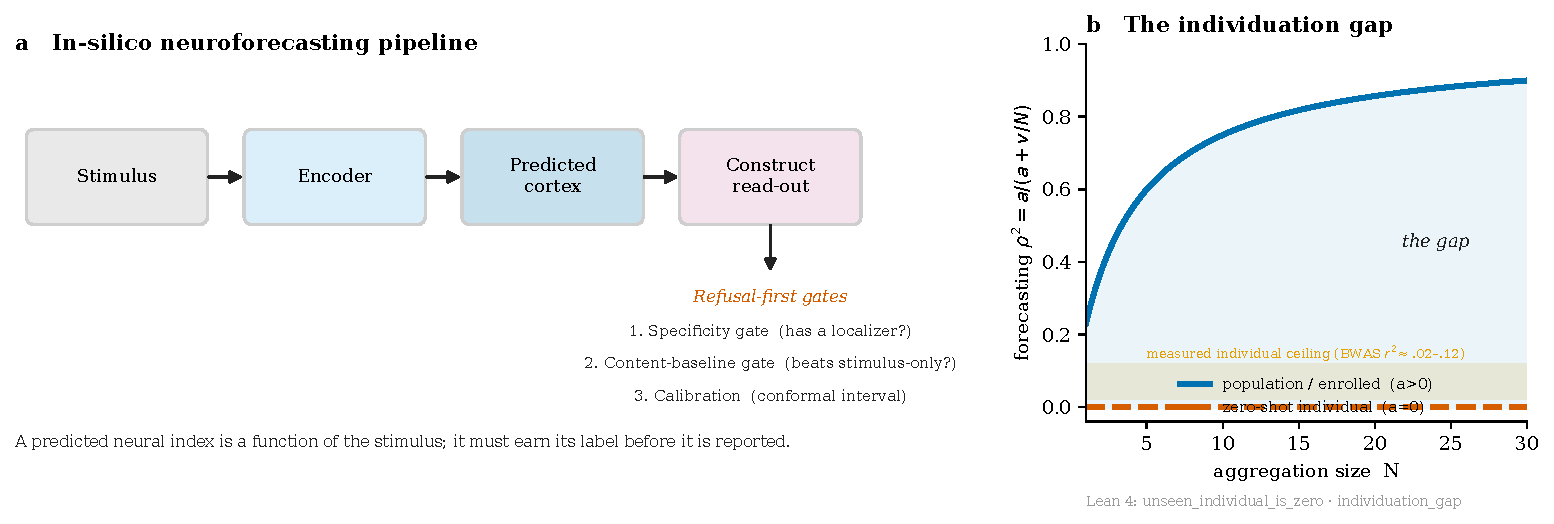
\includegraphics[width=0.93\textwidth]{../figures/fig1_schematic.pdf}
\caption{(a)~The in-silico pipeline and the refusal-first gates. (b)~The individuation gap: the population term rises with aggregation while the zero-shot individual term is pinned at zero, below the small measured individual-difference ceiling (Theorems~\ref{thm:agg}--\ref{thm:gap}).}
\label{fig:schematic}
\end{figure*}

\section{Who, not what}
\label{sec:whowhat}
If the individual term is accessible only through enrollment, what does enrollment actually buy? Across three real paired datasets it buys identity, not behavior (Fig.~\ref{fig:evidence}).

\begin{figure*}[t]
\centering
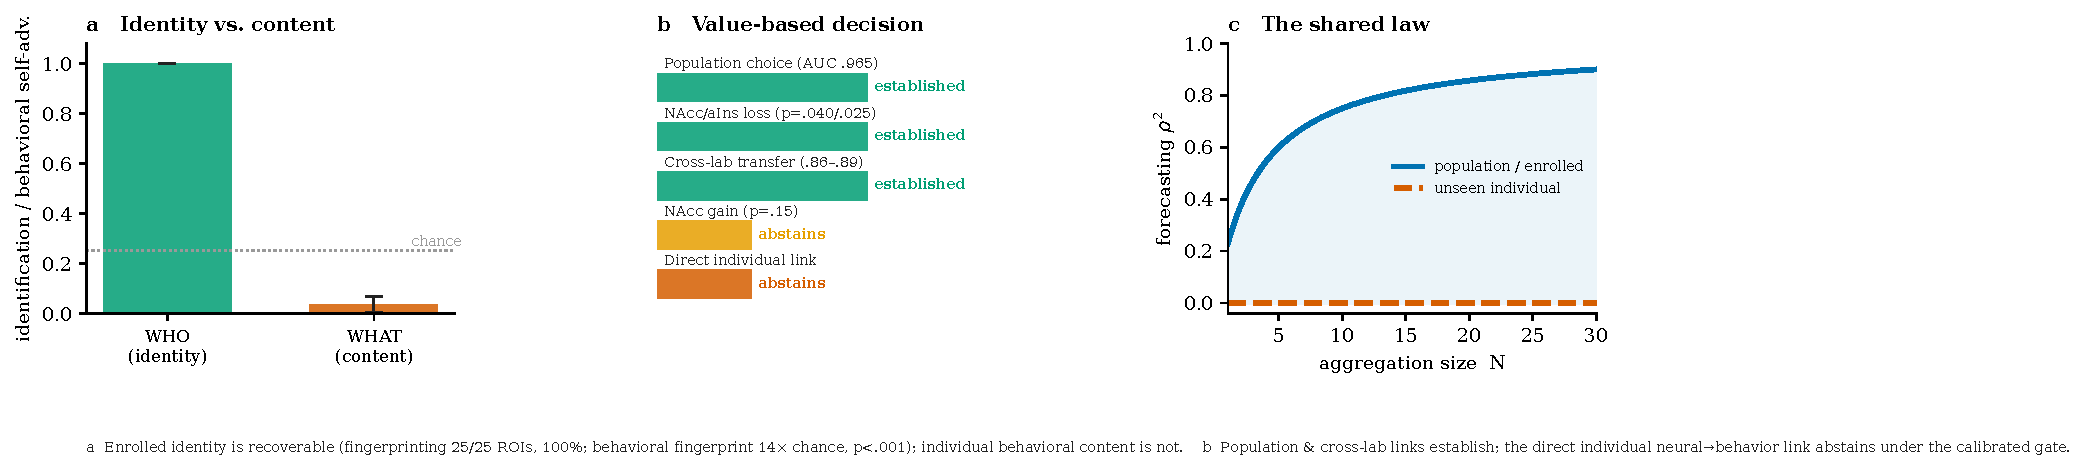
\includegraphics[width=0.93\textwidth]{../figures/fig3_convergent_evidence.pdf}
\caption{Who, not what. (a)~Identity is recoverable (in-scanner fingerprint $100\%$; behavioral fingerprint $14\times$ chance); individual behavioral content is not. (b)~Population and cross-lab links establish; the direct individual link abstains. (c)~Both instantiate the proven gap.}
\label{fig:evidence}
\end{figure*}

\paragraph{Vision encoding (7T fMRI; NSD, BOLD5000).} Subject-specific image-to-fMRI encoders ($N=8$) encode well (median $r$ $0.219$ to $0.463$, all positive). Cross-run fingerprinting identifies the subject in $25/25$ regions at $100\%$ (chance $1/8$): enrolled identity is highly recoverable. The individual geometry that would carry behaviorally relevant content is reliably positive but small ($+0.005$ to $+0.066$ across regions), and the stimulus representation, not the loss, is the ceiling \citep{allen2022,chang2019}.

\paragraph{Value-based decision (fMRI and behavior; NARPS, ds000005).} On $107$ subjects and about $27{,}000$ choices, a behavioral fingerprint identifies individuals at $14\times$ chance ($p=5\times10^{-4}$): identity again recovers. Population links establish (held-out choice AUC $0.965$, conformal coverage $1.00$, ECE $0.034$; loss aversion $\lambda=1.45$ matching \citealp{tom2007}; cross-lab transfer AUC $0.86$ to $0.89$; NAcc and anterior insula track loss, $p=0.040$ and $0.025$). The direct individual neural-to-behavior link abstains under a calibrated minimum-detectable-effect gate \citep{botviniknezer2019}. On the same gambles a content baseline dominates the aggregate, so a predicted index earns no neural credit.

The pattern is consistent: the \emph{who} question (identity, verification) is answerable; the \emph{what} question (this person's mental content or next choice) abstains. Conflating the two is the central error of the personalized-neuro claim.

\section{A Bayes-optimal forecaster cannot escape it}
\label{sec:bayes}
One might hope that a principled probabilistic model recovers the individual where point estimates fail. In the zero-shot regime it does not, and the reason is information-theoretic, not algorithmic. If the predicted feature has no between-subject variance, it is independent of the individual outcome given the population, so the Bayes-optimal individual forecast equals the population forecast and their mutual information is zero.

\begin{proposition}[Zero-shot posterior collapse]
If the predictor is constant across subjects, the posterior over an individual's outcome equals the population prior, and no estimator achieves above-population individual accuracy.
\end{proposition}

We verify this with a Bayesian simulation (sigmoidal choice with a latent per-subject bias; a grid posterior updated from a subject's own trials). At zero-shot the recovery correlation is $r=0.00$ and the incremental AUC over the population model is $+0.000$. Enrollment pays the price: recovery rises to $r=0.58,0.86,0.99$ at $2,10,200$ trials, and the incremental AUC rises to $+0.05,+0.11,+0.14$ and saturates (Fig.~\ref{fig:bayes}). The honest reading is twofold. Zero-shot individual probabilistic prediction is falsified, exactly. Enrolled individual prediction is possible but modest and data-hungry, and it saturates well short of certainty.

\begin{figure}[t]
\centering
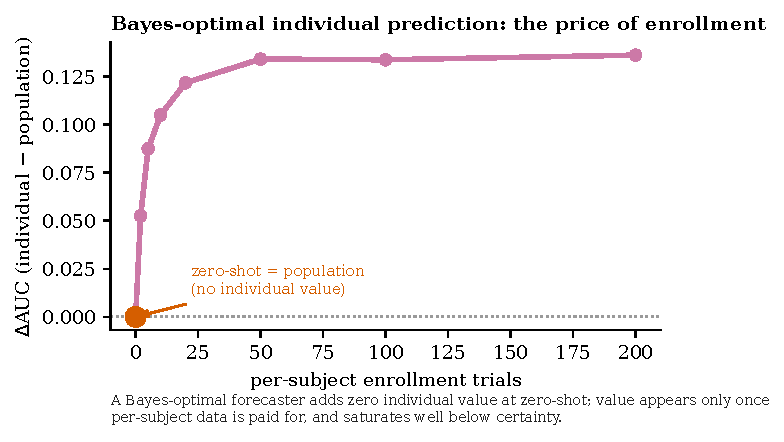
\includegraphics[width=\linewidth]{../figures/fig5_bayes_enrollment.pdf}
\caption{A Bayes-optimal individual forecaster adds exactly zero value at zero-shot and only a modest, saturating gain once per-subject data is paid for.}
\label{fig:bayes}
\end{figure}

\section{Does multimodal fusion rescue it?}
\label{sec:fusion}
A natural rescue is to add EEG, heart rate, electrodermal activity, or hormonal assays. Under independence, inverse-variance fusion lowers variance: the fused variance is at most that of any single modality, a fact we machine-check for the general finite case (\texttt{FusionMath.lean}, \texttt{fused\_le\_min}). The rescue fails in practice because the independence premise does not hold and because each added modality injects its own nuisance variance.

\begin{proposition}[Fusion is not monotone in the number of modalities]
With fused signal $A=\sum_m a_m$ and fused effective noise $v+\sum_m\delta_m$, where $\delta_m$ is the nuisance variance the $m$th modality injects, the individual correlation
$\rho^2 = A/(A+v+\sum_m\delta_m)$
increases when modality $m$ is added if and only if $a_m/\delta_m$ exceeds the current signal-to-noise ratio; low-reliability modalities strictly lower it.
\end{proposition}

Figure~\ref{fig:fusion} shows the consequence: adding high-reliability modalities helps, but low-reliability ones (single-channel autonomic signals, slow and state-dependent hormonal assays) push $\rho^2$ back down. Fusion can lift the population term; it does not supply the between-subject signal the individual term needs, and past a point it hurts.

\begin{figure}[t]
\centering
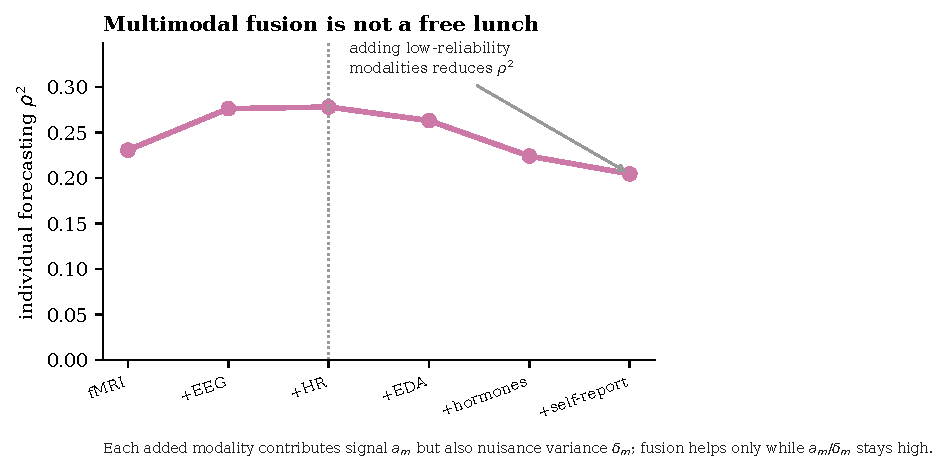
\includegraphics[width=\linewidth]{../figures/fig4_fusion.pdf}
\caption{Multimodal fusion is not a free lunch. Each added modality contributes signal $a_m$ but also nuisance variance $\delta_m$; low-reliability modalities lower individual $\rho^2$.}
\label{fig:fusion}
\end{figure}

\section{Why the individual level is hard}
\label{sec:reliability}
The gap is not an artifact of one pipeline. The field's measurement literature predicts it. Brain-wide association studies have small effect sizes (univariate $r\approx0.14$, multivariate $r\approx0.34$) and need thousands of subjects for reproducibility, while within-person and interventional effects are larger \citep{marek2022,kang2024}. Common task-fMRI individual measures have poor test-retest reliability (mean ICC $0.397$), which bounds any individual-differences use \citep{elliott2020}, though multivariate signatures can do better \citep{kragel2021}. Individual precision functional mapping is achievable but requires hours of per-subject data \citep{gordon2017,du2025}. All three say the same thing as Eq.~\ref{eq:rho}: the individual term is small and expensive, and a zero-shot predictor pays none of the price.

\section{The refusal-first protocol}
\label{sec:protocol}
The practical upshot is a read-out that withholds by default (Fig.~\ref{fig:schematic}a). A construct score is returned only if it passes a specificity gate (the construct term has a meta-analytic localizer and its named regions are the term's best match), a content-baseline gate (the predicted index beats a stimulus-only model out of sample), and a calibration requirement (a split-conformal interval; \citealp{vovk2005}). Separately, the protocol reports identity and content on different channels, so a system may verify \emph{who} without claiming to read \emph{what}. The specificity gate alone withholds, for example, a manipulation index, because no localizer for persuasion exists.

\section{Synthetic validation of the apparatus}
We verify the control ladder recovers known truth before trusting it. In a crossed design (\textsc{world}: signal vs.\ null; \textsc{split}: enrolled vs.\ unseen), with ridge regression, pooled out-of-sample $R^2$, and a paired bootstrap over 20 seeds, Gate~2 (individual value, correct minus wrong subject) fires in exactly the one cell where individual signal exists and the subject is enrolled, with no false positives (Table~\ref{tab:gates}, Fig.~\ref{fig:gates}). In the unseen regime Gate~2 cannot fire, which is Theorem~\ref{thm:zero} in simulation. These numbers are synthetic and validate the apparatus, not any brain.

\begin{table}[t]
\centering\small
\begin{tabular}{@{}llll@{}}
\toprule
World / regime & Gate 1 & Gate 2 & Expected \\
\midrule
\textsc{signal}/enrolled & \textbf{pass} & \textbf{pass} $+0.449$ & fire \\
\textsc{signal}/unseen & no & no $+0.028$ & silent \\
\textsc{null}/enrolled & pass $+0.087$ & no $-0.001$ & silent \\
\textsc{null}/unseen & pass $+0.034$ & no $-0.001$ & silent \\
\bottomrule
\end{tabular}
\caption{Gate~2 fires only where individual signal exists and the subject is enrolled (CI $[+0.378,+0.526]$). Gate~1 passes even in \textsc{null}, so it measures population value and Gate~2 measures individual value.}
\label{tab:gates}
\end{table}

\begin{figure}[t]
\centering
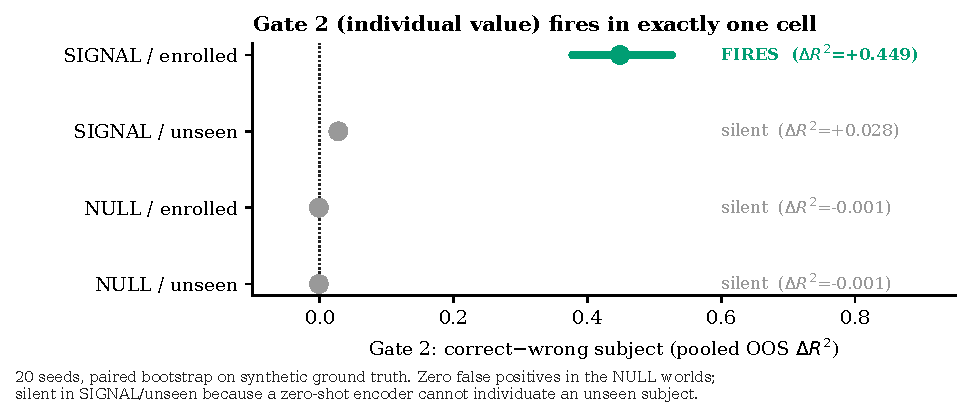
\includegraphics[width=\linewidth]{../figures/fig2_synthetic_gates.pdf}
\caption{Synthetic apparatus check. Gate~2 (individual value) fires only in \textsc{signal}/enrolled; it is silent in both \textsc{null} cells and in \textsc{signal}/unseen.}
\label{fig:gates}
\end{figure}

\section{What would reach the individual level}
The individual mental level is real and causally accessible, but today to invasive methods. Optogenetics achieves cell-type-specific causal control of circuits and behavior, with brain-wide readout when paired with fMRI, in animals \citep{zhao2011,bernalcasas2017}. Intracortical brain-computer interfaces decode attempted speech and movement from a single person's spiking activity at high accuracy and in daily home use \citep{willett2023,card2025,silva2024}. These reach the individual precisely because they record or perturb that individual's own circuitry, which is the between-subject signal a zero-shot non-invasive readout lacks. They mark the direction in which small individual signals may eventually be tracked, and they are out of scope for the non-invasive consumer and clinical claims this paper audits.

\section{Related work}
Measured-brain neuroforecasting \citep{knutson2007,dmochowski2014,yao2024}, reverse-inference caution \citep{poldrack2006,hutzler2013}, conformal prediction \citep{vovk2005}, reliability and sample-size results \citep{marek2022,elliott2020,gordon2017}, and inverse-variance fusion are prior work. The field treats population versus individual as a design trade-off. We argue that for non-invasive and in-silico readouts it is a boundary with a provable shape, separate for identity and content, unrescued by fusion, and enforceable as a protocol.

\section{Limitations}
The synthetic ladder and the Bayesian simulation validate the apparatus and the probability claim, not any specific product. The real-data arms were analyzed under separate protocols in prior work, so they are convergent evidence rather than one preregistered study; the decision-fMRI individual link abstains at the boundary of power, which is an abstention, not a positive null. The fusion proposition is elementary and not machine-checked beyond the independence lemma. Reported numbers were read from the analysis repositories and should be regenerated from frozen commits before camera-ready.

\section{Conclusion}
Non-invasive and in-silico brain readouts can tell you who someone is and can forecast a crowd. They cannot tell you what an individual is thinking or will choose, because the individual signal is not in the input without a per-subject price, and that price currently buys identity rather than behavior. Fusion does not change this, a Bayes-optimal forecaster does not escape it, and the measurement literature already said so. A read-out that respects the boundary returns fewer numbers, and the ones it returns have earned their label.

\begin{thebibliography}{99}\small
\bibitem[Allen et al.(2022)]{allen2022} Allen, E.~J., et al. (2022). A massive 7T fMRI dataset to bridge cognitive neuroscience and artificial intelligence. \emph{Nature Neuroscience}, 25, 116--126.
\bibitem[Bernal-Casas et al.(2017)]{bernalcasas2017} Bernal-Casas, D., et al. (2017). Studying brain circuit function with dynamic causal modeling for optogenetic fMRI. \emph{Neuron}, 93(3), 522--532.
\bibitem[Botvinik-Nezer et al.(2019)]{botviniknezer2019} Botvinik-Nezer, R., et al. (2019). A large-scale fMRI dataset for the study of value-based decision making. \emph{Scientific Data}, 6, 106.
\bibitem[Card et al.(2026)]{card2025} Card, N.~S., et al. (2026). Long-term independent use of an intracortical brain--computer interface for speech and cursor control. \emph{Nature Medicine}, 32(7), 2504--2510.
\bibitem[Chang et al.(2019)]{chang2019} Chang, N., et al. (2019). BOLD5000: a public fMRI dataset of 5000 images. \emph{Scientific Data}, 6, 49.
\bibitem[Dmochowski et al.(2014)]{dmochowski2014} Dmochowski, J.~P., et al. (2014). Audience preferences are predicted by temporal reliability of neural processing. \emph{Nature Communications}, 5, 5567.
\bibitem[Du et al.(2025)]{du2025} Du, J.-N., et al. (2025). Within-individual precision mapping of brain networks exclusively using task data. \emph{Neuron}.
\bibitem[Elliott et al.(2020)]{elliott2020} Elliott, M.~L., et al. (2020). What is the test-retest reliability of common task-fMRI measures? \emph{Psychological Science}, 31(7), 792--806.
\bibitem[Genevsky et al.(2017)]{genevsky2017} Genevsky, A., Yoon, C., \& Knutson, B. (2017). When brain beats behavior: neuroforecasting crowdfunding outcomes. \emph{Journal of Neuroscience}, 37(36), 8625--8634.
\bibitem[Gordon et al.(2017)]{gordon2017} Gordon, E.~M., et al. (2017). Precision functional mapping of individual human brains. \emph{Neuron}, 95(4), 791--807.
\bibitem[Hutzler(2013)]{hutzler2013} Hutzler, F. (2013). Reverse inference is not a fallacy per se. \emph{NeuroImage}, 84, 1061--1069.
\bibitem[Kang et al.(2024)]{kang2024} Kang, K., et al. (2024). Study design features increase replicability in brain-wide association studies. \emph{Nature}, 636(8043), 719--727.
\bibitem[Knutson et al.(2007)]{knutson2007} Knutson, B., et al. (2007). Neural predictors of purchases. \emph{Neuron}, 53(1), 147--156.
\bibitem[Kragel et al.(2021)]{kragel2021} Kragel, P.~A., et al. (2021). Functional MRI can be highly reliable, but it depends on what you measure. \emph{Psychological Science}, 32(4), 622--626.
\bibitem[Marek et al.(2022)]{marek2022} Marek, S., et al. (2022). Reproducible brain-wide association studies require thousands of individuals. \emph{Nature}, 603, 654--660.
\bibitem[Poldrack(2006)]{poldrack2006} Poldrack, R.~A. (2006). Can cognitive processes be inferred from neuroimaging data? \emph{Trends in Cognitive Sciences}, 10(2), 59--63.
\bibitem[Silva et al.(2024)]{silva2024} Silva, A.~B., et al. (2024). The speech neuroprosthesis. \emph{Nature Reviews Neuroscience}, 25, 473--492.
\bibitem[Tom et al.(2007)]{tom2007} Tom, S.~M., et al. (2007). The neural basis of loss aversion in decision-making under risk. \emph{Science}, 315(5811), 515--518.
\bibitem[Vovk et al.(2005)]{vovk2005} Vovk, V., Gammerman, A., \& Shafer, G. (2005). \emph{Algorithmic Learning in a Random World}. Springer.
\bibitem[Willett et al.(2023)]{willett2023} Willett, F.~R., et al. (2023). A high-performance speech neuroprosthesis. \emph{Nature}, 620, 1031--1036.
\bibitem[Yao et al.(2024)]{yao2024} Yao, X., et al. (2024). Using neural data to forecast aggregate consumer behavior in neuromarketing. \emph{Journal of Consumer Behaviour}.
\bibitem[Zhao et al.(2011)]{zhao2011} Zhao, S., et al. (2011). Cell type-specific channelrhodopsin-2 transgenic mice for optogenetic dissection of neural circuitry function. \emph{Nature Methods}, 8(9), 745--752.
\end{thebibliography}

\end{document}
